\begin{frame}[plain]
\frametitle{Switch Data Planes today}
Two key decisions on a per-packet basis:
\begin{itemize}
\item Scheduling: Which packet should be sent out next?
\item[]
\item Queue Management: How long can queues grow? Which packet to drop?
\item[]
\end{itemize}
\end{frame}

\begin{frame}[plain]
\frametitle{The long lineage of in-network algorithms}
\begin{center}
\noindent \hspace{-.75 cm} \includegraphics[width=.9\textwidth]{march-4.png}
\end{center}
\end{frame}


\begin{frame}[plain]
\frametitle{The long lineage of in-network algorithms}
\begin{center}
\noindent \hspace{-.75 cm} \includegraphics[width=.9\textwidth]{march-3.png}
\end{center}
\end{frame}

\begin{frame}[plain]
\frametitle{The long lineage of in-network algorithms}
\begin{center}
\noindent \hspace{-.75 cm} \includegraphics[width=.9\textwidth]{march-2.png}
\end{center}
\end{frame}

\begin{frame}[plain]
\frametitle{The long lineage of in-network algorithms}
\begin{center}
\noindent \hspace{-.75 cm} \includegraphics[width=.9\textwidth]{march-1.png}
\end{center}
\end{frame}

\begin{frame}[plain]
\frametitle{The long lineage of in-network algorithms}
\begin{center}
\noindent \hspace{-.75 cm} \includegraphics[width=.9\textwidth]{march.png}
\end{center}
\end{frame}

\begin{frame}[plain]
\frametitle{The Data Plane is continuously evolving}
\begin{itemize}
\item Each scheme wins in its own evaluation

\item[]

\item Some believe in a ``silver bullet'' knobless in-network method

\end{itemize}
\end{frame}

\begin{frame}[plain]
\frametitle{We disagree: There is no silver bullet!}
\begin{itemize}
\item{Different applications care about different objectives}

\item[]
%%\begin{itemize}
%%\item Interactive video conferencing apps need both high throughput \& low delay.
%%\item Bulk transfers care only about high throughput.
%%\item Web browsers care about minimizing flow completion time (FCT).
%%\end{itemize}

\item{Applications use different transport protocols}
\item[]
%%%\begin{itemize}
%%%\item Some respond to loss, e.g., TCP Cubic, TCP NewReno.
%%%\item Others respond to packet inter-arrival times, e.g., WebRTC, LEDBAT.
%%%\item Others respond to per-packet delay, e.g., TCP Vegas.
%%%\item Yet others respond to both delay and packet loss, e.g., Compound TCP.
%%%\end{itemize}

\item{Networks are diverse and heterogeneous}

%%\begin{itemize}
%%\item High-speed, low-latency, Data Center networks
%%\item Low-speed, high-latency, transcontinental links
%%\item High-speed, high-variability, bufferbloated LTE links
%%\end{itemize}
%\item{``One size fits all'' is overly constraining.}
\end{itemize}
\end{frame}

\begin{frame}[plain]
\frametitle{Early symptoms}
\begin{itemize}
\item{Hard to configure wired AQM for wireless links}

\item[]

\item{Several distinct in-network schemes for datacenters}
\begin{itemize}
\item DCTCP, HULL, D3, DeTail, PDQ, pFabric
\end{itemize}

\item[]

\item{No consensus on the ``right metric"}
\begin{itemize}
\item Minimizing missed deadlines
\item Flow Completion Time
\item Latency
\item Throughput
\item Tail Latency
\item \dots 
\end{itemize}

\end{itemize}
\end{frame}

\begin{frame}[plain]
\frametitle{Quantifying ``No Silver Bullet'': Network Configurations}
\begin{table}
\begin{tabular}{|p{0.25\linewidth}|p{0.73\linewidth}|}
\hline
{\bf \underline{Configuration}} & {\bf \underline{Description}} \\
&\\
{\bf CoDel+FCFS} & One shared FCFS queue with CoDel\\
& \\
%\hline
{\bf CoDel+FQ} & Per-flow fair queueing with CoDel on each queue\\ 
&\\
%\hline
{\bf Bufferbloat+FQ} & Per-flow fair queueing with deep buffers on
each queue\\ 
& \\
\hline
\end{tabular}
\end{table}
\end{frame}

\begin{frame}[plain]
\frametitle{Quantifying``No Silver Bullet'': Workloads and Objectives}

\begin{table}
\begin{tabular}{|p{0.18\linewidth}|p{0.37\linewidth}|p{0.38\linewidth}|}
\hline
{\bf \underline{Workload}} & {\bf \underline{Description}} & {\bf \underline{Objective}} \\
& &\\
\textbf{\emph{Bulk}} & Long-running TCP flow & Maximize throughput \\
& &\\
\textbf{\emph{Web}} & Switched TCP flow with ON and OFF periods &
Minimize 99.9 \%ile flow completion time \\
& &\\
\textbf{\emph{Interactive}} & Long-running real-time
streaming app & Maximize $\frac{\mbox{throughput}}{\mbox{delay}}$, i.e.,
  ``power'' \\ 
& &\\
\hline
\end{tabular}
\end{table}
\end{frame}

\begin{frame}[plain]
\frametitle{Quantifying ``No Silver Bullet''}
\begin{center}
\includegraphics[width=\columnwidth]{fig-6.pdf}
\end{center}
\end{frame}

\begin{frame}[plain]
\frametitle{Quantifying ``No Silver Bullet''}
\begin{center}
\includegraphics[width=\columnwidth]{fig-5.pdf}
\end{center}
\end{frame}

\begin{frame}[plain]
\frametitle{Quantifying ``No Silver Bullet''}
\begin{center}
\includegraphics[width=\columnwidth]{fig-4.pdf}
\end{center}
\end{frame}

\begin{frame}[plain]
\frametitle{Quantifying ``No Silver Bullet''}
\begin{center}
\includegraphics[width=\columnwidth]{fig-3.pdf}
\end{center}
\end{frame}

\begin{frame}[plain]
\frametitle{Quantifying ``No Silver Bullet''}
\begin{center}
\includegraphics[width=\columnwidth]{fig-2.pdf}
\end{center}
\end{frame}

\begin{frame}[plain]
\frametitle{Quantifying ``No Silver Bullet''}
\begin{center}
\includegraphics[width=\columnwidth]{fig-1.pdf}
\end{center}
\end{frame}

\begin{frame}[plain]
\frametitle{Quantifying ``No Silver Bullet''}
\begin{center}
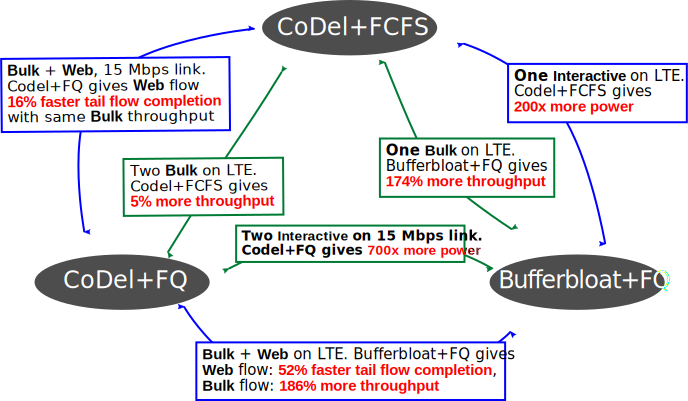
\includegraphics[width=\columnwidth]{fig.pdf}
\end{center}
\end{frame}

\begin{frame}[plain]
\frametitle{Why is no single data plane configuration the best?}
\begin{itemize}
\item Bufferbloat on variable-rate links helps throughput!
      \begin{itemize}
      \item Variable-rate links have an inherent delay-throughput tradeoff
      \end{itemize} 

\item[] 

\item FCFS is preferable to Fair Queuing in some cases
      \begin{itemize}
      \item When equally aggressive flows compete, they don't need
        protection from each other
        \item Helps reduce tail packet delay
      \end{itemize}

\item[]

\item Fair Queuing is required in some cases
      \begin{itemize}      
      \item When competing flows aren't equally aggressive,
        isolation helps
      \end{itemize}
\end{itemize}
\end{frame}

\begin{frame}[plain]
\frametitle{So what should the network designer do?}
Architect a flexible data plane
\begin{itemize}
\item Implement in-network queue management and scheduling in a
  programmable way
\item Not just for selecting among pre-built choices, but to change
  behavior in the field
\item Because there is no silver bullet and innovation will continue!
\end{itemize}
\end{frame}

\begin{frame}[plain]
\frametitle{Controlled flexibility: Want performance, security,
  reliability}

(Or, why this isn't the same as ``active networks'')

\begin{itemize}
\item Provide interfaces to the head and tail of queues
\item Operators specify only queue-management/scheduling logic
\item Code size limits constrain program sophistication
\item No access to packet payloads (for now)
\end{itemize}
\end{frame}

\begin{frame}[plain]
\frametitle{Building such a data plane in four parts}
\begin{itemize}
\item Hardware gadgets (primitives)
      \begin{itemize}
      \item Random number generators (RED, BLUE)
      \item Binary tree of comparators (pFabric, SRPT)
      \item EWMA estimators (RED, AVQ, CSFQ)
      \end{itemize}

\item I/O interfaces
      \begin{itemize}
      \item Drop/mark head/tail of queue
      \item Interrupts for enqueue/dequeue
      \item Read packet headers
      \end{itemize}

\item State maintenance
      \begin{itemize}
      \item Per-flow (WFQ, DRR)
      \item Per-src address (PF)
      \item For fastest flows alone (AFD)
      \end{itemize}

\item A domain-specific instruction set
      \begin{itemize}
      \item Expresses control flow
      \item Implements new functions unavailable in hardware
      \end{itemize}
\end{itemize}
\end{frame}

\begin{frame}[plain]
\frametitle{Example implementation: CoDel}
\begin{center}
\includegraphics[width=\columnwidth]{codel.pdf}
\end{center}
\begin{center}
Synthesis numbers on Xilinx Kintex-7: \\
\begin{tabular}{lll}
\bf Resource & \bf Usage & \bf Fraction of FPGA \\
\hline Slice logic & 1,256 & 1\% \\
Slice logic dist. & 1,975 & 2\% \\
IO/GTX ports & 27 & 2\% \\
DSP slices & 0 & 0\% \\
Maximum speed & 12.9 $\times 10^6$ pkts/s \\
\end{tabular}
\end{center}
\end{frame}

\begin{frame}[plain]
\frametitle{Limitations and Practical Considerations:}
\begin{itemize}
\item Cannot express several network functions that need payloads.
\item How do applications signal objectives to the network?
\item Feasibility at 10G on high port-density  switches.
\item Mechanism to map flows onto per-port queues.
\item Energy and Area overheads.
\end{itemize}
\end{frame}

\begin{frame}[plain]

\frametitle{Related Work}
\begin{itemize}

\item Active Networks
\item[]

\item Software Routers
\item[]

\item Software-Defined Networking
\item[]

\end{itemize}
\end{frame}

\begin{frame}[plain]

\frametitle{Conclusion}
\begin{itemize}

\item There is no silver bullet to in-network resource control because
  of application and network diversity

\item[]
\item Algorithms will continue to evolve: the data plane should help

\item[]
\item Extending SDN to the data plane in a thoughtful manner is a good
  research direction with potentially high real-world impact

\end{itemize}
\end{frame}
